\subsection{Traffic Demand Per Subscriber}\label{subsec:behavior}

\begin{figure}[t]
\begin{minipage}{1\linewidth}
\centering
%
\begin{subfigure}[b]{1\linewidth}
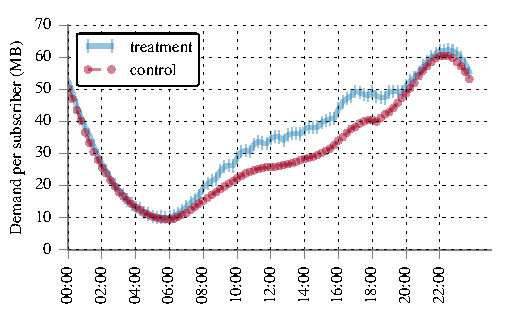
\includegraphics[width=\linewidth]{figures/weekday_demand_mean.pdf}
               \caption{Weekday traffic demand.\label{fig:weekday-daily-usage}}
\end{subfigure}
%
\begin{subfigure}[b]{1\linewidth}
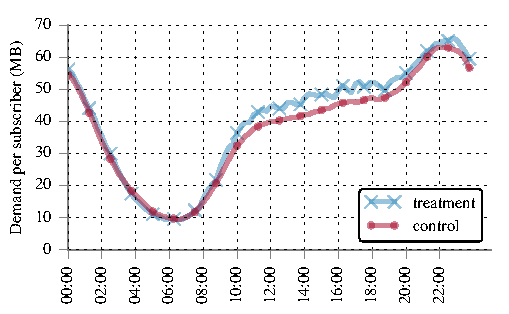
\includegraphics[width=\linewidth]{figures/weekend_demand_mean.pdf}
               \caption{Weekend traffic demand.\label{fig:weekend-daily-usage}}
\end{subfigure}
%
\end{minipage}
\caption{Mean subscriber demand (bytes per 15-minute interval).}
\label{fig:traffic-demand-timeseries}
\end{figure}


\begin{table}[t]
\centering
\begin{tabular}{ cc | ccc }\\\hline
                         &           & median & mean  & 95\%  \\\hline
\multirow{2}{*}{Weekday} & treatment & 35.97  & 35.58 & 61.12 \\
                         & control   & 28.06  & 31.12 & 58.78 \\\hline
\multirow{2}{*}{Weekend} & treatment & 45.27  & 40.10 & 64.27 \\
                         & control   & 41.15  & 37.66 & 62.23 \\\hline
\end{tabular}
\caption{Weekday and weekend traffic demand patterns.}
\label{tab:traffic-demand-description}
\end{table}

We first explore how an upgrade to a higher service tier affected the
average traffic demand per subscriber, for different times of the day
and days of the week.  Figure~\ref{fig:traffic-demand-timeseries} shows
the average downlink traffic demand across subscribers for a week, for
both the treatment and control groups. We observe that subscriber
behavior differs significantly on weekdays and weekends.  The average
per subscriber demand over a weekday is 35.6 MB, and the 95th percentile
peak demand is 61.12 MB for subscribers in the treatment group
(Table~\ref{tab:traffic-demand-description}).  Over a weekend, the
average demand is 40.1 MB, and the 95th percentile demand is 64.3 MB for
treatment, but the median is 45.27 MB due to consistent use in the major
part of the day.  On weekdays, traffic demand increases monotonically
from morning until prime-time hours in the evening. On weekends, we
observed a sharp rise in demand in the early morning period, from 8:00
a.m. to 10:00 a.m.. Then, the demand plateaued until the next rise
during before evening prime-time hours. Previous reports indicate that
the aggregate traffic volume for US fixed access link providers usually
troughs during mid-afternoon hours (between
2:00~p.m.--6:00~p.m.)~\cite{sandvine20141h}. \f{In contrast to these
  previous reports, we do not observe such troughs in 
subscriber demand.}

\begin{figure}[t]
\begin{minipage}{1\linewidth}
\centering
%
%\begin{subfigure}[b]{.33\linewidth}
%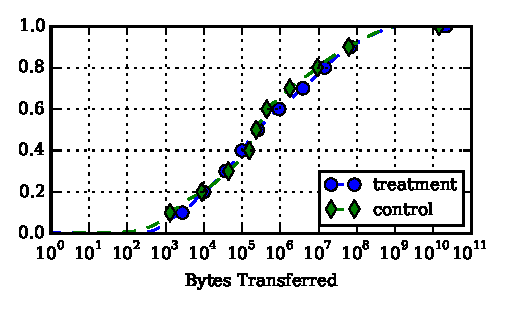
\includegraphics[width=\linewidth]{figures/cdf-all-bytes.pdf}
%                \caption{Overall traffic demand for all subscribers at all times\label{fig:CDF-data-rate}}
%\end{subfigure}
% maybe should be mean per day?
%
\begin{subfigure}[b]{1\linewidth}
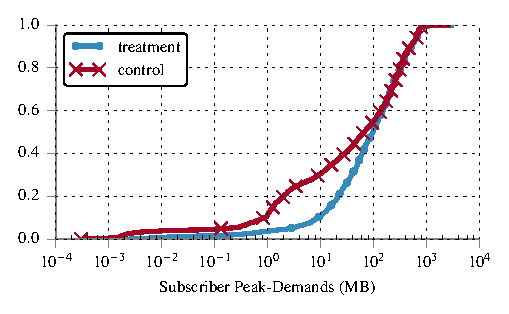
\includegraphics[width=\linewidth]{figures/cdf_peak_demand-overall.pdf}
               \caption{Peak (95\%) traffic demand per subscriber\label{fig:CDF-data-rate-perc95}}
\end{subfigure}

\begin{subfigure}[b]{1\linewidth}
% 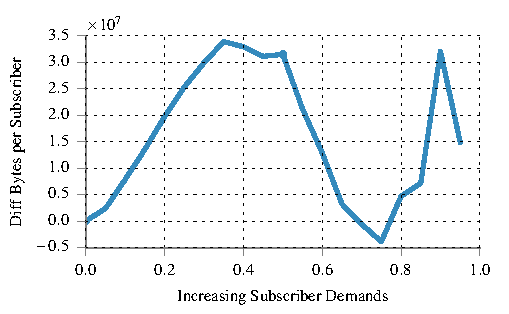
\includegraphics[width=\linewidth]{figures/diff_perc95_bytes_subsc-overall.pdf}	% 5 percentile
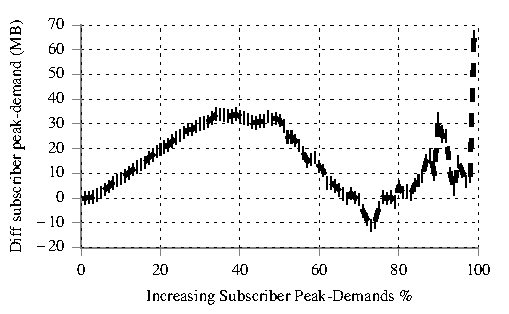
\includegraphics[width=\linewidth]{figures/diff_perc95_bytes_subsc-overall_01.pdf}		% 1 percentile
               \caption{
                 Change in overall peak (95\%) demand per subscriber. y-axis unites
                  are bytes transferred in the peak 15-minute
                  interval, in MB.
 \label{fig:diff-peak-overall}}
\end{subfigure}
%
\end{minipage}
\caption{95th percentile traffic demand (bytes per 15 minutes) per
  subscriber for the control and treatment groups. \label{fig:traffic-demand-overall}}
\end{figure}

% Figure \ref{CDF-data-rate} shows the data rate for each measurement period and every subscriber.
Figure \ref{fig:CDF-data-rate-perc95} shows the distribution of the the
95th percentile downlink traffic demand over the three-month measurement
period. The highest peak demand per 15-minute interval amongst
subscribers in the control group was 2.97 GB; in the treatment group,
the highest peak demand was 3.0 GB.
The average peak traffic demand was 169.8 MB for \control{} and
186.6 MB for \treatment{}. Given the 105 Mbps service-tier capacity,
this means that users even on averaging the 95th percentile demand,
users rarely utilize their links (average utilization was 1.43\%
for \control{} and 1.5\% for \treatment{})

We suspected that the subscribers who downloaded most bytes in the
higher service tier would be the ones causing the largest difference in
mean demand, as previous studies have observed such a phenomenon. \f{In
  fact, we observed that the more moderate subscribers actually seemed
  to exhibit larger differences in traffic deman: The median peak demand
  was 66.7 MB for the lower service tier, and 98.4 MB for the higher
  tier.  This result indicates that the more moderate subscribers in the
  control group who received a service-tier upgrade significantly
  altered their peak demand.}  We also observed a significant difference
in the mean peak demand was also present in the 50\% of
subscribers in the control group with the lowest traffic demand when
compared to the same set of subscribers of the treatment group. (This
disparity appears as a large gap under the 50\% tick in
Figure~\ref{fig:CDF-data-rate-perc95}.)


Figure~\ref{fig:diff-peak-overall} shows another way of looking at this
phenomenon: it explores users with particular traffic demands in the
control and treatment groups change their peak demand in response to the
upgrade.  For each group, we sort the subscribers according to
increasing demand.  Then we compute the difference in peak demand for
each percentile in the group.  For example, the plot shows the median
user (50\% on the x-axis) increased their peak demand by about 25\% in
response to the service tier upgrade.  Comparing the 70\% subscribers of
both groups with the least demand, we see that peak demand in the
treatment group is higher than the peak demand in the control group,
indicating that in fact even moderate users increase their demand as a
result of the service-tier increase, even though they are not using the
full capacity in either case.
When we combine this analysis with that in
Figure~\ref{fig:CDF-data-rate-perc95}, we find that these subscribers
who respond with increased usage have a peak demand less than 200~MB.
Naturally, the small number of users with the highest demand (closer to
100\%) also tend to increase their usage, sometimes substantially.


\if 0
\begin{figure}[t]
\centering
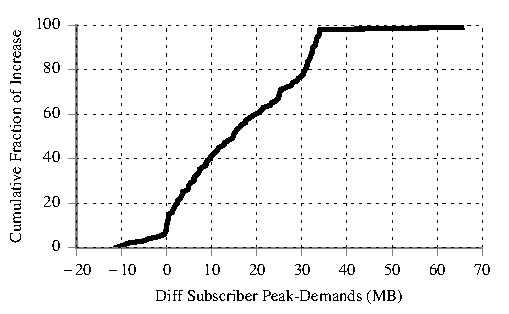
\includegraphics[width=\linewidth]{figures/cdf_diff_perc95_bytes_subsc-overall.pdf}
               \caption{Distribution of the difference between \treatment{} and \control{}
               peak traffic demands\label{fig:cdf-diff-perc95}}
\end{figure}

Figure~\ref{fig:cdf-diff-perc95} shows the distribution of the
difference in demands of the two groups by percentile. There are 15\%
subscribers in the \treatment{} that have peak demands have peak demands
that are similar, or lower than the equivalent 15\% of subscribers in
\control{}. Figure~\ref{fig:diff-peak-overall} shows that this group
lies around between the 65 and 80 percentile
demand. Figure~\ref{fig:CDF-data-rate-perc95} shows that between the
65-80 percentile mark, subscribers had a demand between 200~MB to
400~MB. For these subscribers in the treatment group, the equivalent
subscribers in the control group had demands upto 10~MB higher. 20\% of the
differences between the peak of the treatment group and the control
group are higher than 30 MB. These subscribers lie between the between
30\% and 50\% difference. Their peak demands are between between 40--100
MB as part of the higher tier, and 10--70~MB if they belong to the lower
tier.  The subscribers with the highest traffic demand in the treatment
group (beyond 800 MB peak demand) have demands 15--30~MB more than the
highest peak demanding subscribers in the control group.  In the case of
upstream traffic, 90\% of users in the treatment group consistently
upload 2 MB more traffic than the control group. The top 10\% of the
highest demanding subscribers in the treatment group uploaded between 2--10~MB
more than the top 10\% of the control group.
\fi

\begin{figure}[t]
\begin{minipage}{1\linewidth}
\centering
\begin{subfigure}[b]{1\linewidth}
 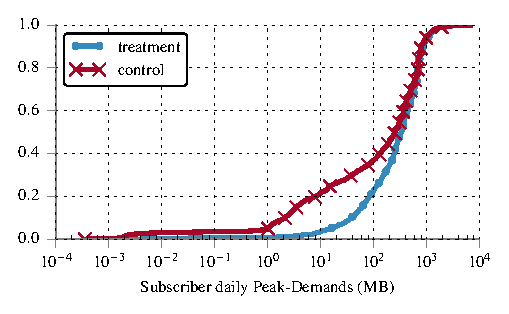
\includegraphics[width=\linewidth]{figures/cdf_peak_demand-daily.pdf}
                \caption{Peak (95\%) traffic demand per subscriber\label{fig:CDF-data-rate-daily-perc95}}
 \end{subfigure}
\begin{subfigure}[b]{.99\linewidth}
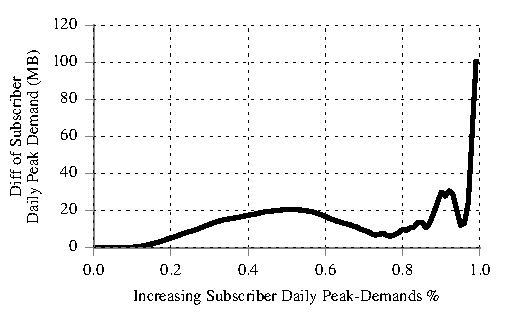
\includegraphics[width=\linewidth]{figures/diff_perc95_bytes_subsc-daily-overall_01.pdf}		%1 percentile
%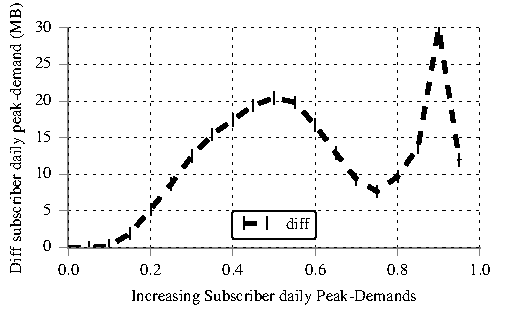
\includegraphics[width=\linewidth]{figures/diff_perc95_bytes_subsc-daily-overall.pdf}		%5 percentile
                \caption{Change in daily peak (95\%) demand per subscriber. y-axis unites
                  are bytes transferred in the peak 15-minute
                  interval, in MB.\label{fig:diff-peak-daily}} 
\end{subfigure}
%
\end{minipage}
  \caption{Difference between peak-demands of subscribers from \treatment{} and
  \control{} groups. Subscribers were considered at every 5\% in each
  group. 
  \label{fig:traffic-demand-daily}}
\end{figure}


\f{Further investigation revealed that users with moderate traffic
  demands not only increase their traffic demands in aggregate, but also
  on a daily basis.}  Figure~\ref{fig:traffic-demand-daily} shows that
when subscribers on the lower tier had a daily peak demand under 600~MB,
70\% of subscribers in the treatment group had 15-minute demands that
were 5--20~MB higher.  The ratio of the the differences in demand across
percentiles also shows that the 40\% of subscribers with lowest peak
demands in the control group more than
double their daily peak traffic demand in response to service-tier upgrades.

\f{One possible explanation for why moderate users increase their usage
  in response to a service-tier upgrade is that the higher service tier
  not only affords more capacity, but also a better user experience
  (\eg, faster downloads).  Thus, even though users may not be
  exhausting the capacity of the higher service tier, they nonetheless
  seem to respond to the service tier upgrade by using the Internet more
  than they had before the service-tier upgrade.}


\if 0
There could be many reasons for this increase in demand for subscribers with
lower peak demands. One reason could be short term web activities (such as short videos,
web browsing) that have a slightly higher traffic demand. Such an increase in demand would
then be apparent during hours when users pursue such activities (mostly prime-time).
Another reason could be an increase in background traffic (such as software updates).
Studying the applications responsible for such behavioral changes in traffic demand is not
in the scope of our current work. However, an interesting question that arises is: when
does the demand increase the most throughout a day? Our analysis showed that the most
subscribers reach within 95\% of daily maximum demand between 8:00 p.m.--12:00 a.m.
\fi

% \begin{table}[h]
% \begin{tabular}{lllll}
%         &           & 1     & 2     & 3     \\
% Weekday & treatment & 21:45 & 00:00 & 23:30 \\
%         & control   & 22:30 & 22:15 & 00:00 \\
% Weekend & treatment & 23:30 & 23:45 & 14:30 \\
%         & control   & 22:30 & 21:30 &      
% \end{tabular}
% \end{table}